
\subsubsection{Displacement simulation}\label{sec:DisplacementSimulation}
The effect of data qubit displacement was considered in the proposal \cite{OGorman2016} using a simulation of the logical surface code operations, where the authors derived a code threshold for displacements of $R=\SI{6.1}{\nano\metre}$. We will now look more closely at the magnitude and character of errors that happen from displacements close to this threshold. 

We ran 800 simulations for even parity with no bit-flips, and 800 for odd parity with a randomly chosen bit-flip. The full dynamics of the interaction Hamiltonian derived in section \ref{sec:dipole-dipole} was simulated for each run, with randomly generated qubit displacements within the pillbox region illustrated in fig.\@ \ref{fig:pillbox} for $R = \SI{6}{\nano\metre}$, within the \SI{6.1}{\nano\metre} derived threshold. Finally, to ensure the full scheme as proposed was being implemented, randomly chosen twirling operations were added.

The 1600 simulation runs consumed 96 computer-hours, yielding the histogram in fig.\@ \ref{fig:DisplacementHistogram}. Two peaks are observed, with no significant deviation from $\pi$/$2\pi$, but the standard deviations of \num{0.265+-0.001} yield rotations from the mean of up to $\tfrac{\pi}{4}$, corresponding to a \SI{14.6}{\percent} error rate for the worst case simulated.

The standard deviation in phase represents \SI{4.2}{\percent} of $2\pi$, within the \SI{4.4}{\percent} phase jitter the proposal \cite{OGorman2016} used to derive the effect of probe jitter from the logical surface code simulation. However, projecting onto the $x$-axis to find the probability of measuring $\ket{+}\big/\ket{-}$, we find that the mean measurement success probability is \SI{98.27}{\percent} for both even and odd parity. This corresponds to a measurement error rate of \SI{1.7}{\percent}, above the code threshold of \SI{1.1}{\percent} for the surface code \cite{Wang2011,Fowler2012} despite the $R = \SI{6}{\nano\metre}$ displacement simulated being within the $R=\SI{6.1}{\nano\metre}$ threshold derived using logical simulations in the proposal \cite{OGorman2016}. 

From these simulations we conclude that the large $\tfrac{1}{r^3}$ dependence in the interaction strength has a strong enough effect on phase accumulation to bring the measurement success rate below the code threshold for the surface code. This brings into doubt the claim in the proposal \cite{OGorman2016} that the code is tolerant to physically plausible qubit displacements, and more work will be needed to resolve this and potentially calculate a new threshold.

%Thus we can conclude that, though the interaction strength has a high $\tfrac{1}{r^3}$ dependence, the parity measurement appears surprisingly tolerant to qubit displacement. Additionally, with the phase variance at the code threshold for qubit displacement being within the phase jitter parameter implemented in the proposal's logical simulations, the results of their simulation likely hold true for many likely qubit implantation techniques with precisions within the $R=\SI{6.1}{\nano\metre}$. % THIS IS BULLSHIT




\begin{figure}
	\centering
	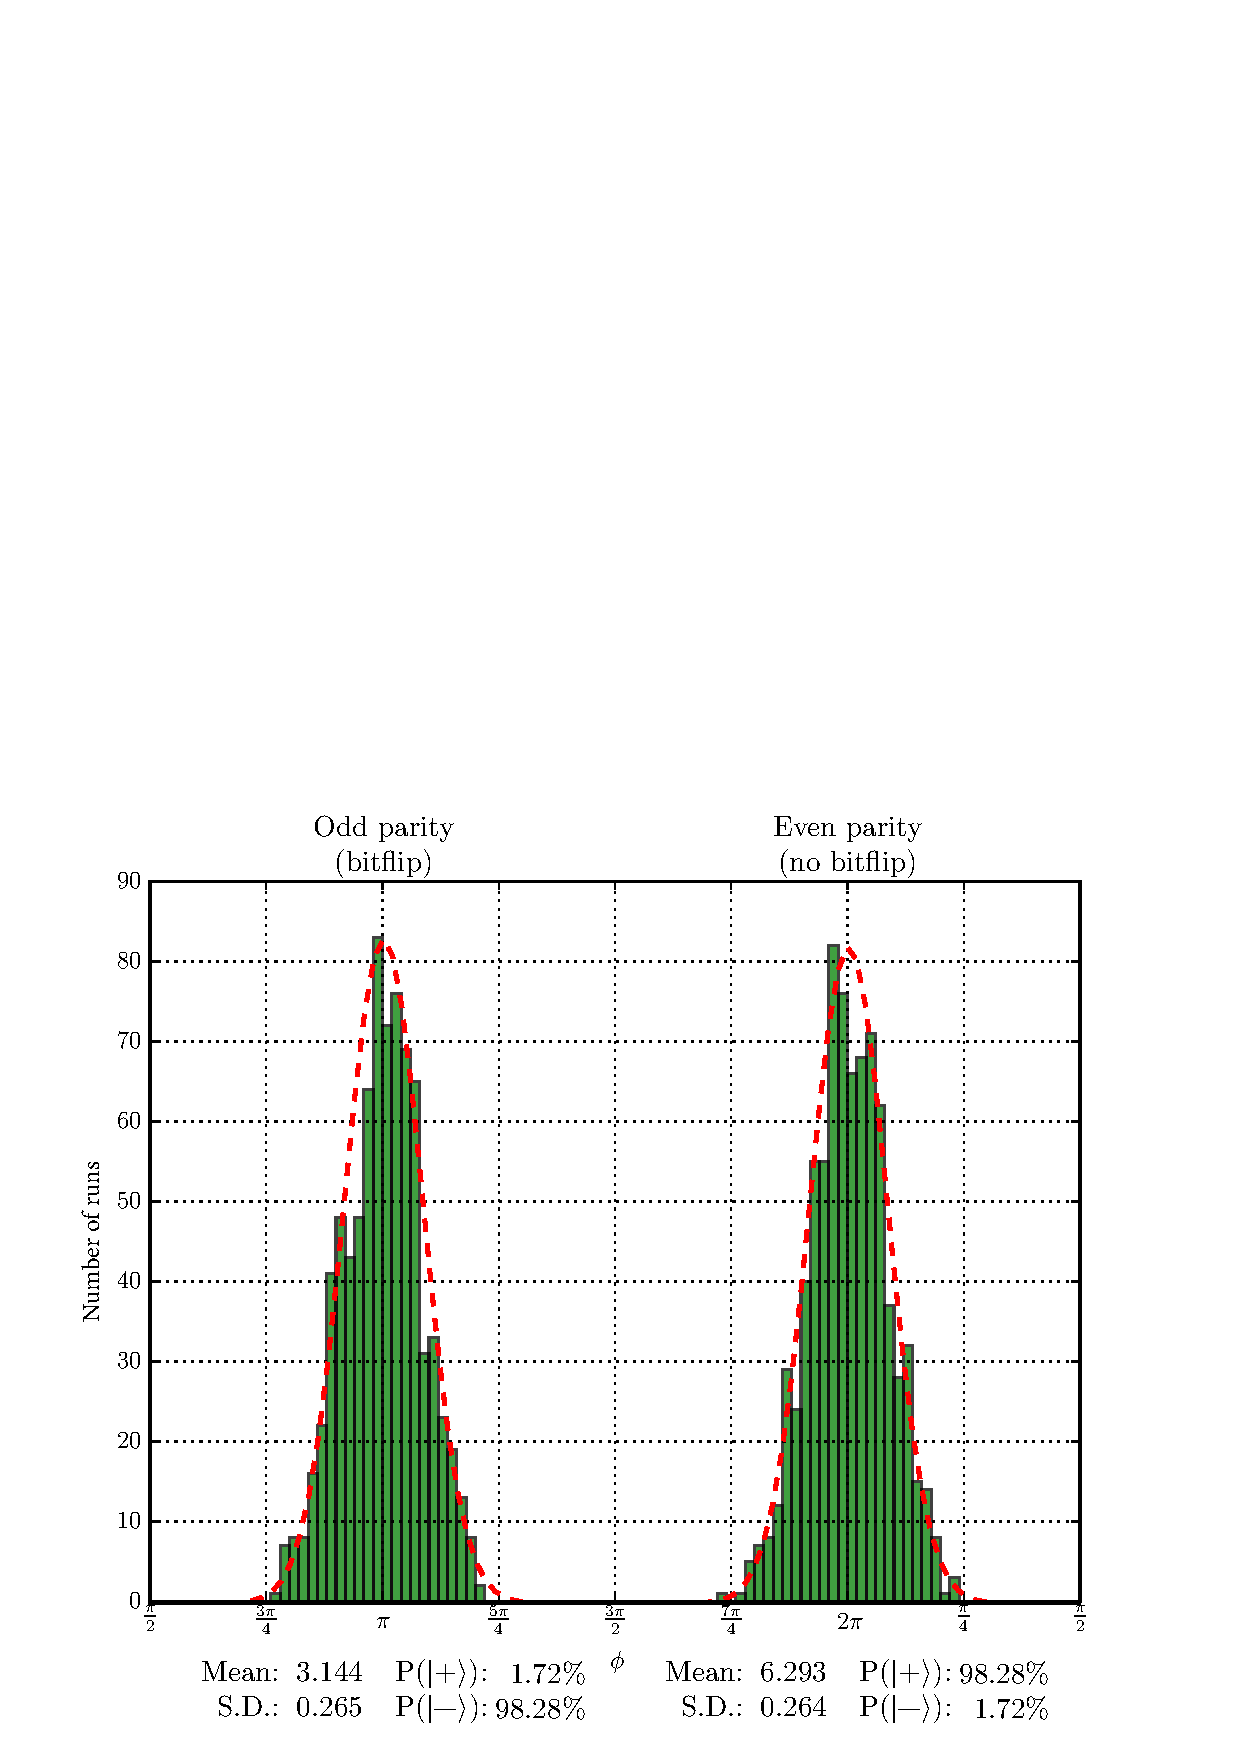
\includegraphics[width=\columnwidth]{../Figures/Displacement_Histogram.pdf}	
	\caption{Histogram of 1600 simulation runs given random qubit displacements generated within the pillbox of fig.\@ \ref{fig:pillbox} with $R = \SI{6}{\nano\metre}$ with random twirling operations applied. The resultant measurement success probabilities \SI{98.28}{\percent} are not within the \SI{1.1}{\percent} surface code error threshold \cite{Wang2011,Fowler2012}, suggesting further work may be required to characterise the code's tolerance of qubit displacements. }
	\label{fig:DisplacementHistogram}
\end{figure}